%
% hauptwerte-residuen.tex -- Hauptwerte mit dem Residuentheorem
%
% !TEX root = ../../buch.tex
% !TEX encoding = UTF-8
%
\section{Hauptwerte mit dem Residuentheorem
\label{hauptwert:section:hauptwerte-residuen}}
\kopfrechts{Hauptwerte mit dem Residuentheorem}


\subsection{Ein Integral ohne Polstelle auf der Achse
\label{hauptwert:subsection:aufwaermbeispiel}}
%
% halbkreis-ohne-pol.tex
%
% (c) 2026 Damien Flury, OST Ostschweizer Fachhochschule
%
\begin{figure}
\centering
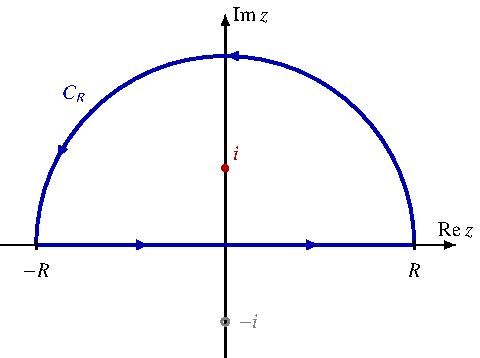
\includegraphics{papers/hauptwert/images/halbkreis-ohne-pol.pdf}
\caption{Halbkreiskontur ohne Polstelle auf der reellen Achse.
Der geschlossene Weg besteht aus der Strecke $[-R,R]$ und dem grossen
Halbkreis $C_R$ und wird im positiven Sinn durchlaufen.
Von den beiden Polstellen von $1/(1+z^2)$ liegt einzig $i$ im umlaufenen
Gebiet, während $-i$ in der unteren Halbebene keinen Beitrag liefert.
\label{hauptwert:figure:halbkreis-ohne-pol}}
\end{figure}


Als nächstes betrachten wir das uneigentliche Integral
\begin{equation}
  \int_{-\infty}^{\infty} \frac{1}{1 + x^2}\,dx.
\end{equation}

In der reellen Analysis kennt man dazu die Stammfunktion $\arctan$ und
kommt mit
\begin{equation}
  \int_{-\infty}^{\infty} \frac{1}{1 + x^2}\,dx
  =
  \lim_{a\to\infty}
  \Bigl[
    \arctan(x)
  \Bigr]_{-a}^{a}
  =
  \lim_{a\to\infty} 2\arctan(a)
  =
  \pi
  \label{hauptwert:equation:arctan}
\end{equation}
ohne Umweg über die komplexe Ebene zum Ziel, wie in
Abschnitt~\ref{buch:integration:residuen:section:beispiel} vorgerechnet.

Die Strecke $[-R,R]$ lässt sich mit dem grossen Halbkreis $C_R$ zu einem
geschlossenen Weg ergänzen
(Abbildung~\ref{hauptwert:figure:halbkreis-ohne-pol}).
Wäre der Integrand im umlaufenen Gebiet holomorph, dann wäre dieses
Wegintegral nach dem
Satz~\ref{buch:integration:wegintegral:satz:zusammenziehbar} gleich $0$.
Setzt man die Funktion jedoch in die komplexe Ebene fort, dann fällt auf,
dass sie zwei Polstellen hat, denn
\begin{equation}
  f(z)
  =
  \frac{1}{1 + z^2}
  =
  \frac{1}{(z - i)(z + i)}
  \label{hauptwert:equation:faktorisierung}
\end{equation}
wird für $z_1 = i$ und $z_2 = -i$ singulär.
Von den beiden liegt einzig $z_1 = i$ im umlaufenen Gebiet.

Das Wegintegral ist daher nicht $0$, sondern wird allein durch das Residuum
in $z_1$ bestimmt.
Nach Satz~\ref{buch:analytisch:laurent:residuum:satz} ist dieses Residuum
der Quotient aus dem Zähler und der Ableitung des Nenners,
\begin{equation}
  \res(z_1;f)
  =
  \biggl.\frac{1}{(1 + z^2)'}\biggr|_{z = i}
  =
  \frac{1}{2i},
  \label{hauptwert:equation:residuum-i}
\end{equation}
und mit \eqref{buch:analytisch:laurentreihen:residuum:eqn:integralres}
folgt für jedes $R > 1$
\begin{equation}
  \int_{-R}^{R} f(x)\,dx
  +
  \int_{C_R} f(z)\,dz
  =
  2\pi i \cdot \frac{1}{2i}
  =
  \pi.
  \label{hauptwert:equation:aufwaermkontur}
\end{equation}


\subsection{Satz vom kleinen Kreisbogen
\label{hauptwert:subsection:halbresiduen}}
%
% halbkreiskontur.tex
%
% (c) 2026 Damien Flury, OST Ostschweizer Fachhochschule
%
\begin{figure}
\centering
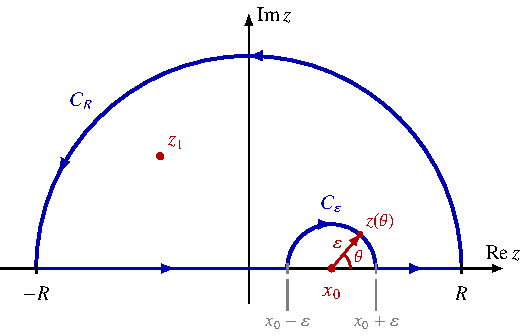
\includegraphics{papers/hauptwert/images/halbkreiskontur.pdf}
\caption{Halbkreiskontur zur Berechnung von Hauptwerten.
Die Kontur wird im positiven Sinn durchlaufen und besteht aus den beiden
Strecken auf der reellen Achse, der Einbuchtung $C_\varepsilon$ oberhalb der
Polstelle $x_0$ und dem grossen Halbkreis $C_R$.
Die Einbuchtung schliesst $x_0$ aus dem umlaufenen Gebiet aus und wird
dabei im negativen Sinn durchlaufen;
eingeschlossen wird nur der Pol $z_1$ in der oberen Halbebene.
\label{hauptwert:figure:halbkreiskontur}}
\end{figure}

Man betrachte ein Integral von einer beliebigen reellen Funktion mit einer
Singularität an einem Punkt $x_0$ (z.B. $\int_{a}^{b} \frac{1}{x}\,dx$). Da das
direkte Integrieren durch $x_0$ nicht funktioniert, weicht man über die
komplexe Ebene der Singularität aus und macht einen kleinen Bogen darum
(Abbildung~\ref{hauptwert:figure:halbkreiskontur}).
\begin{lemma}
\label{hauptwert:lemma:halbresiduen}
Man integriere eine Funktion $f(z)$ mit Polstelle erster Ordnung in $x_0$
entlang einer Kurve $C_\varepsilon$, wobei $C_\varepsilon$ einen kleinen Halbkreis
über die Polstelle an $x_0$ von $x_0-\varepsilon$ nach $x_0+\varepsilon$ macht.
Es gilt
\begin{equation}
  \lim_{\varepsilon \to 0^+} \int_{C_\varepsilon} f(z)\,dz = -i\pi \res(x_0;f).
\end{equation}
\end{lemma}

\begin{proof}
Da $f$ in $x_0$ eine Polstelle erster Ordnung hat, lässt sich $f$ in einer
Umgebung von $x_0$ nach Satz~\ref{buch:analytisch:laurent:satz:laurentreihe}
als
\begin{equation}
  f(z) = \frac{\res(x_0;f)}{z - x_0}
       + \underbrace{g(z)}_{\text{Taylorreihe}}
  \label{hauptwert:halbresiduen:zerlegung}
\end{equation}
schreiben, wobei $g$ in dieser Umgebung holomorph und damit auf einer
kompakten Umgebung von $x_0$ durch ein $M$ beschränkt ist.
Der Halbkreis $C_\varepsilon$ wird gemäss
Abbildung~\ref{hauptwert:figure:halbkreiskontur} durch
\begin{equation}
  z(\theta) = x_0 + \varepsilon e^{i\theta},
  \qquad \theta\colon \pi \to 0,
  \qquad dz = i\varepsilon e^{i\theta}\,d\theta
\end{equation}
  parametrisiert, er wird also im negativen Sinn (Uhrzeigersinn) durchlaufen.
Für den ersten Term in \eqref{hauptwert:halbresiduen:zerlegung} kürzt sich
$\varepsilon e^{i\theta}$ weg und es bleibt
\begin{equation}
\begin{aligned}
  \int_{C_\varepsilon} \frac{\res(x_0;f)}{z - x_0}\,dz
  &= \int_{\pi}^{0} \frac{\res(x_0;f)}{\varepsilon e^{i\theta}}
     \, i\varepsilon e^{i\theta}\,d\theta \\
  &= i\,\res(x_0;f) \int_{\pi}^{0} d\theta \\
  &= -i\pi \res(x_0;f),
\end{aligned}
\end{equation}
unabhängig von $\varepsilon$.
Der Beitrag von $g$ verschwindet dagegen im Grenzübergang, denn die Länge
von $C_\varepsilon$ ist $\pi\varepsilon$ und damit
\begin{equation}
  \biggl| \int_{C_\varepsilon} g(z)\,dz \biggr|
  \le M \pi \varepsilon
  \longrightarrow 0
  \qquad (\varepsilon \to 0^+).
\end{equation}
Zusammen folgt die Behauptung.
\end{proof}


\subsection{Das Lemma von Jordan
\label{hauptwert:subsection:jordan}}
%
% jordan-ungleichung.tex
%
% (c) 2026 Damien Flury, OST Ostschweizer Fachhochschule
%
\begin{figure}
\centering
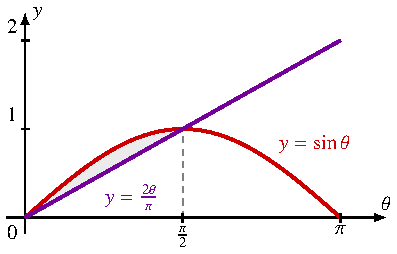
\includegraphics{papers/hauptwert/images/jordan-ungleichung.pdf}
\caption{Auf dem Intervall $[0,\frac{\pi}{2}]$ verläuft der Sinusbogen
oberhalb seiner Sehne, es gilt also $\sin\theta \ge \frac{2\theta}{\pi}$.
Beide Kurven treffen sich in den Endpunkten $0$ und $\frac{\pi}{2}$.
\label{hauptwert:figure:jordan-ungleichung}}
\end{figure}


\begin{lemma}
\label{hauptwert:lemma:jordan}
Sei $a > 0$ und $C_R$ ein Halbkreis in der oberen Halbebene mit Radius $R$.
Geht $f(z)$ für $|z| \to \infty$ gleichmässig gegen $0$, gilt also
\begin{equation}
  M(R) = \max_{z \in C_R} |f(z)| \longrightarrow 0
  \qquad (R \to \infty),
  \label{hauptwert:equation:jordanbedingung}
\end{equation}
dann ist
\begin{equation}
  \lim_{R \to \infty} \int_{C_R} f(z) e^{i a z}\,dz = 0.
\end{equation}
\end{lemma}

Die Bedingung \eqref{hauptwert:equation:jordanbedingung} ist insbesondere
für Funktionen der Form $\frac{P}{Q}$ mit $\deg Q > \deg P$ erfüllt.

\begin{proof}
  Der Bogen $C_R$ wird durch
  $z(\theta) = R e^{i \theta}$, $\theta\colon 0 \to \pi$, mit
  $dz = i R e^{i \theta}\,d\theta$ parametrisiert, was
  \begin{equation}
    \int_{C_R} f(z) e^{iaz}\,dz
    =
    \int_{0}^{\pi} f(R e^{i \theta}) e^{i a R e^{i \theta}} i R e^{i \theta}\,d\theta
  \end{equation}
  ergibt.

  Als nächstes betrachten wir den Betrag und erhalten
  \begin{equation}
    \biggl| \int_{C_R} f(z) e^{iaz}\,dz \biggr|
    \le
    \int_{0}^{\pi}
      \bigl| f(Re^{i\theta}) \bigr|
      \bigl| e^{iaRe^{i\theta}} \bigr|
      \bigl| i R e^{i \theta} \bigr|
      \,d\theta.
  \end{equation}
  Nach Voraussetzung~\eqref{hauptwert:equation:jordanbedingung} ist
  $|f(Re^{i\theta})| \le M(R)$, und wegen $|i| = |e^{i\theta}| = 1$ ist
  $|iRe^{i\theta}| = R$.
  Da weder $M(R)$ noch $R$ von $\theta$ abhängen, können sie vor das
  Integral gezogen werden,
  \begin{equation}
    \biggl| \int_{C_R} f(z) e^{iaz}\,dz \biggr|
    \le
    R\,M(R) \int_{0}^{\pi} \bigl| e^{iaRe^{i\theta}} \bigr| \,d\theta.
    \label{hauptwert:equation:jordanabschaetzung}
  \end{equation}

  Für den Betrag einer Exponentialfunktion ist allein der Realteil des
  Exponenten entscheidend, denn der Imaginärteil trägt wie gerade gesehen mit
  $|e^{i\theta}| = 1$ nichts bei.
  Mit $z = R\cos\theta + iR\sin\theta$ wird
  \begin{equation}
    iaz
    =
    -aR\sin\theta + i\,aR\cos\theta
    \qquad\Longrightarrow\qquad
    \bigl| e^{iaz} \bigr| = e^{-aR\sin\theta}.
    \label{hauptwert:equation:jordandaempfung}
  \end{equation}
  Hier werden beide Voraussetzungen gebraucht: auf dem oberen Halbkreis ist
  $\sin\theta \ge 0$, wegen $a > 0$ ist der Exponent daher negativ und der
  Faktor gedämpft.
  An den beiden Endpunkten $\theta = 0$ und $\theta = \pi$, wo der Bogen
  die reelle Achse trifft, ist er allerdings gleich $1$ und dämpft nichts.

  Das verbleibende Integral ist symmetrisch bezüglich
  $\theta \mapsto \pi - \theta$, und auf $[0,\frac{\pi}{2}]$ verläuft der
  Sinusbogen oberhalb seiner Sehne
  (Abbildung~\ref{hauptwert:figure:jordan-ungleichung})
  \cite[Abschnitt~81]{hauptwert:brown-churchill},
  \begin{equation}
    \sin\theta \ge \frac{2\theta}{\pi},
    \label{hauptwert:equation:jordanungleichung}
  \end{equation}
  womit der Integrand durch eine Exponentialfunktion mit linearem Exponenten
  nach oben abgeschätzt werden kann,
  \begin{equation}
  \begin{aligned}
    \int_{0}^{\pi} e^{-aR\sin\theta}\,d\theta
    &= 2 \int_{0}^{\pi/2} e^{-aR\sin\theta}\,d\theta
     \le 2 \int_{0}^{\pi/2} e^{-2aR\theta/\pi}\,d\theta \\
    &= 2 \Bigl[
         -\frac{\pi}{2aR} e^{-2aR\theta/\pi}
       \Bigr]_{0}^{\pi/2}
     = \frac{\pi}{aR}\bigl(1 - e^{-aR}\bigr)
     \le \frac{\pi}{aR}.
  \end{aligned}
  \end{equation}
  Eingesetzt in \eqref{hauptwert:equation:jordanabschaetzung} hebt sich das
  $R$ der Weglänge gegen das $R$ im Nenner weg,
  \begin{equation}
    \biggl| \int_{C_R} f(z) e^{iaz}\,dz \biggr|
    \le
    R\,M(R) \cdot \frac{\pi}{aR}
    =
    \frac{\pi}{a} M(R),
  \end{equation}
  und da $M(R) \to 0$ nach Voraussetzung
  \eqref{hauptwert:equation:jordanbedingung} gilt, verschwindet auch die
  linke Seite für $R \to \infty$
  \cite{hauptwert:qncubed3-jordan}.
\end{proof}


\subsection{Die Halbkreiskontur
\label{hauptwert:subsection:halbkreiskontur}}

\begin{satz}
\label{hauptwert:satz:hauptformel}
Damit der Residuensatz funktioniert, werden vier Voraussetzungen benötigt:
\begin{enumerate}
  \item $f$ ist innerhalb des Integrationsweges holomorph (d.h. überall differenzierbar) bis auf endlich viele Singularitäten.
  \item $f$ hat maximal Singularitäten ersten Grades $x_1,\dots,x_m$ auf dem reellen Bereich.
  \item In der oberen Halbebene hat $f$ endlich viele Polstellen $z_1,\dots,z_n$.
  \item Das Integral des grossen Bogens $C_R$ verschwindet für $R \to \infty$:
  \begin{equation}
  \lim_{R \to \infty} \int_{C_R} f(z)\,dz = 0.
  \label{hauptwert:equation:bogenbedingung}
  \end{equation}
\end{enumerate}

Sind diese Voraussetzungen erfüllt, dann gilt
  \begin{equation}
    \pv \int_{-\infty}^{\infty} f(x)\,dx = 2 i \pi \sum_{k=1}^{n} \res(z_k; f) + i \pi \sum_{j=1}^{m} \res(x_j; f).
  \end{equation}
\end{satz}

\begin{proof}
\end{proof}


\subsection{Ein Warnbeispiel
\label{hauptwert:subsection:warnbeispiel}}
